\section{Results: useful readiness, bounded advantage}
\subsection{A working capability; conventional reuse explains the gain}
All 288 calibration and 432 confirmation batches qualified under the frozen predicate. Confirmation includes 3,024 right-hand sides and 288 additional preflight columns. No planned confirmation batch was dropped or replaced; no budget stop occurred. Table~\ref{tab:numerical} reports the primary $q=16$ comparison. Figure~\ref{fig:frontier} shows how the paid preparation stage changes the response deadline that can be met.

\begin{table}[ht]\centering\small
\begin{tabular*}{\linewidth}{@{\extracolsep{\fill}}lrrrrr@{}}\toprule
& \multicolumn{3}{c}{Full batch median wall time (ms)} & \multicolumn{2}{c}{Paired median ratio}\\
Matrix & Repeated & Cached & Certified & Repeated/cert. & Cert./cached\\\midrule
1138\_bus & 25.234 & 2.538 & 3.608 & 7.00 & 1.44\\
bcsstk14 & 522.091 & 41.534 & 42.495 & 12.32 & 1.02\\
bcsstk18 & 4056.292 & 292.803 & 298.746 & 13.60 & 1.01\\
bcsstk24 & 941.448 & 71.915 & 77.429 & 12.24 & 1.09\\
\bottomrule\end{tabular*}
\caption{\obs{}. Twelve held-out paired blocks per matrix, 16 right-hand sides. ``Repeated'' is the setup ablation. ``Cached'' is conventional reuse with identical acceptance checks. Full batch time includes preparation and checking; shared campaign overhead is separately retained. Paired ratios need not equal ratios of the displayed medians.}
\label{tab:numerical}\end{table}

The instrument saves a mean 0.0212, 0.4813, 3.7556 and 0.8692 seconds relative to repeated setup in matrix order; all four paired timing intervals exclude zero. Against conventional reuse, it adds preflight and recipe work, and the median full-batch ratio exceeds one on every matrix. Some mean differences cross zero under timing noise; that does not establish a systematic solver improvement. The strongest numerical method found is ordinary factor reuse with fresh output checks, with the recipe and evidence layer added when traceability is required.

The certified ready-stage medians at $q=16$ are 1.083, 7.479, 37.882 and 15.122 milliseconds. These condition on factors and right-hand sides already being available. Their preparation has not vanished from the cost ledger. The matrix-specific plots are a measured readiness frontier on this host, not an extrapolation to larger problems or a guarantee that an industrial deadline will be met.

\begin{figure}[ht]\centering
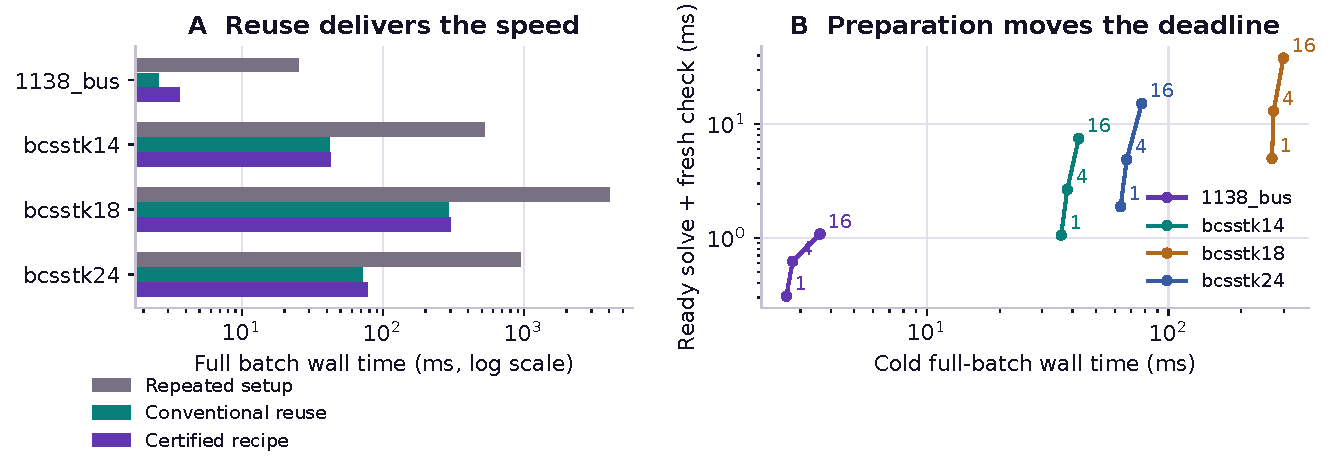
\includegraphics[width=\linewidth]{figures/readiness_frontier.pdf}
\caption{\obs{}. (A) Primary-count full-batch medians. (B) Certified full-batch cost versus ready solve-and-check latency; point labels are right-hand-side counts 1, 4 and 16. Connecting lines guide the eye between tested counts only. Both factors and synthetic right-hand sides exist at the ready-stage origin. Preparation is paid.}
\label{fig:frontier}\end{figure}

An independently written numerical checker recomputed 24 saved solution columns using explicit CSR sums and checked the logged criteria, source/data identities and accounting partitions across the full result ledger. Its supplemental audit passed 11,988 checks. This is implementation independence within the same research workflow, not independent institutional certification. The bounded CG diagnostic did not qualify on any of the four confirmation cases within 400 iterations; those results are retained rather than promoted as a new superiority claim over tuned iterative methods.

\subsection{Forecast skill resolves locally; adoption does not}
The preregistered primary deadline multiplier 1 yields Brier 0.072056 versus 0.259971 for the calibration-only pooled constant, across 720 correlated outcomes. The paired block interval for the score difference is $[-0.191480,-0.184338]$. Across all three deadline multipliers, the secondary score is 0.031463 versus 0.242373 on 2,160 correlated outcomes. The complete 180-target ledger was frozen before confirmation. Figure~\ref{fig:calibration} keeps these scopes separate.

The probabilities are not perfectly calibrated. Beta smoothing leaves the largest extreme bins underconfident, and intermediate bins are small. Conditioning on method, deadline and readiness distinguishes largely easy and hard local timing events; the constant comparator is weak. The result supports H3 for this narrow target, without establishing forecast skill across hosts, future workloads, scientific adoption or the intelligence transition itself. No external accepted-delivery probability was issued or scored as a success.

\begin{figure}[ht]\centering
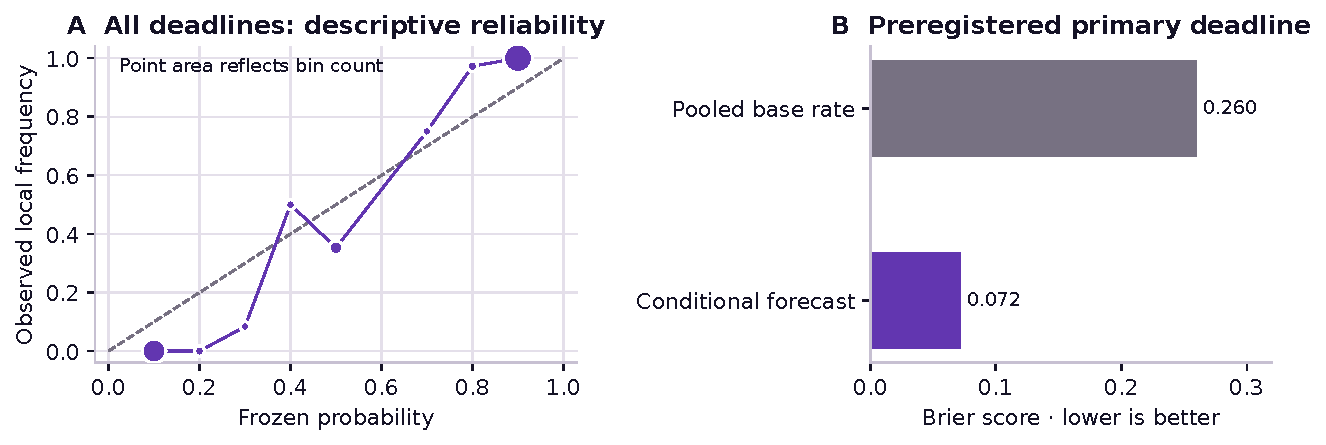
\includegraphics[width=\linewidth]{figures/calibration.pdf}
\caption{\obs{} outcomes of \pend{} forecasts issued before execution. (A) Descriptive reliability across all three declared deadline multipliers; correlated repeated targets and unequal bin counts limit interpretation. (B) Primary deadline score on 720 outcomes; the secondary all-deadline aggregate is shown separately. The baseline is a pooled calibration-only constant, not a specialist forecasting competitor.}
\label{fig:calibration}\end{figure}

\subsection{The timing policy does not establish unique net advantage}
The calibration-selected comparator is \texttt{static\_expert}, a fixed calibrated rule with permissible adaptive arrival recourse, not an observed human expert. The confirmation retains 32,256 policy rows over 4,608 paired worlds. An independently implemented audit reconstructs policy choices, probabilities, value of information, costs, block summaries and primary bootstrap intervals: 1,776,489 checks pass. It cannot reconstruct exact first-qualified timestamps that were not separately logged; it verifies the event bounds available in the retained fields.

\begin{figure}[ht]\centering
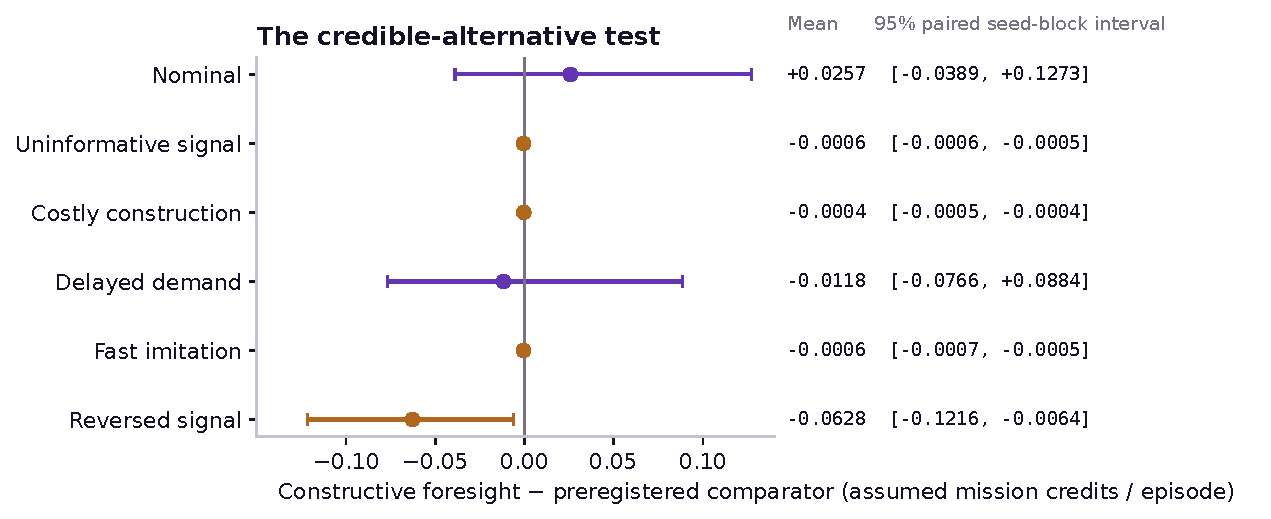
\includegraphics[width=\linewidth]{figures/causal_comparison.pdf}
\caption{\simu{}. Constructive foresight minus the locked calibrated fixed rule; one assumed credit per qualified on-time request and one credit per common clock unit of accounted cost. Intervals resample 24 complete seed blocks within each regime. They describe Monte Carlo variation under the stated model, not uncertainty about real markets or adoption. Tiny negative gaps in three regimes reflect extra controller work.}
\label{fig:causal}\end{figure}

The nominal effect is $+0.025667$ assumed credits per episode, with interval $[-0.038950,0.127277]$. The positive point estimate is too uncertain to establish the preregistered positive comparative claim. Delayed demand produces $-0.011762$ with an interval crossing zero. Reversed signal likelihood produces $-0.062780$, interval $[-0.121571,-0.006446]$. In the uninformative, costly-construction and fast-imitation regimes, native decisions and deliveries tie the fixed rule, while repeated deliberation adds small cost. H2 is therefore not established.

More decisively, the conventional compiled same-information policy has zero action disagreements with constructive foresight across all 4,608 worlds. Mean accepted counts are identical in every regime, while mean controller cost is lower. Its equal-regime advantage over constructive foresight is 0.000548 assumed credits per episode, interval $[0.000534,0.000565]$. This is a small computational efficiency difference, not an economic windfall. Equal information and an equally capable builder eliminate a unique-policy advantage claim in this tested model.

Constructive foresight does outperform the deliberately limited forecast-only and wait-then-build policies in the equal-weight descriptive aggregate. That contrast shows why these weak ablations are insufficient as the sole evidence for advantage. Appendix~\ref{app:comparisons} reports all eligible-comparator differences. No regime weighting was learned from confirmation; equal weighting is an analytic summary, not an estimate of industry prevalence.

The uninformative-signal control leads constructive foresight to buy no signal. Nominal acquisition occurs in 15.23\% of episodes. When a signal cannot change the best feasible action, its acquisition cost has no decision benefit. Eighty late attempts remain in the complete policy ledger with their consumed work charged; latent future service durations are never available to admission decisions. A forecast that becomes false after distribution change is retained as a failed prediction, not rewritten as a successful intervention.

\begin{figure}[ht]\centering
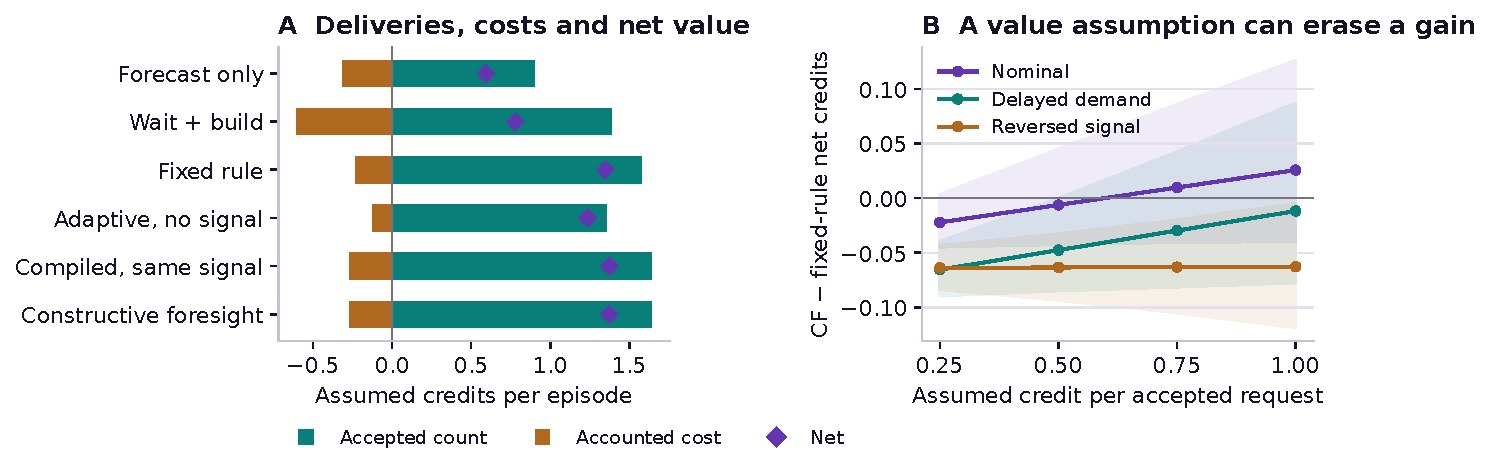
\includegraphics[width=\linewidth]{figures/value_decomposition.pdf}
\caption{\simu{} and \assum{}. (A) Nominal accepted counts, modeled accounted costs and net credits. Numerical wall times, assumed signal/competitor time and measured controller/preparation CPU use one explicit credit rate; they are not dollars or a measured CPU total. (B) Exploratory post-confirmation accounting sensitivity on the same fixed actions and outcomes: reducing assumed service value can erase the nominal gain. Shaded intervals are paired seed-block intervals; this is not a demand-elasticity or market-price forecast.}
\label{fig:value}\end{figure}

\subsection{Restoration works; permission and overhead remain real}
The fixed native demonstration completes initial construction and actual recipe restoration on 1138\_bus with four manufactured right-hand sides. Both outputs pass the separate checker. Restoration preserves parent lineage while returning no active authority, no current proof and no enabled execution. Fresh checking and a separate explicit public-fixture grant are required for the second inspection. Eight native refusal probes and six receiver refusals have the expected outcomes. The corrupted-output negative control fails proof before admission. These observations support H4 only for the tested published paths and fixture.

The complete native process costs 6.552 seconds wall and 6.427 seconds child CPU. Inside the two runs, orchestration and retention consume 2.392 and 3.156 seconds; their numerical handlers take 0.0093 and 0.0063 seconds. Provenance is not free. For kernels this small, a full lifecycle transaction around every solve would dominate useful work. Batching evidence at a justified capability boundary is a plausible engineering improvement, not a measured gain claimed by this study.

\begin{figure}[ht]\centering
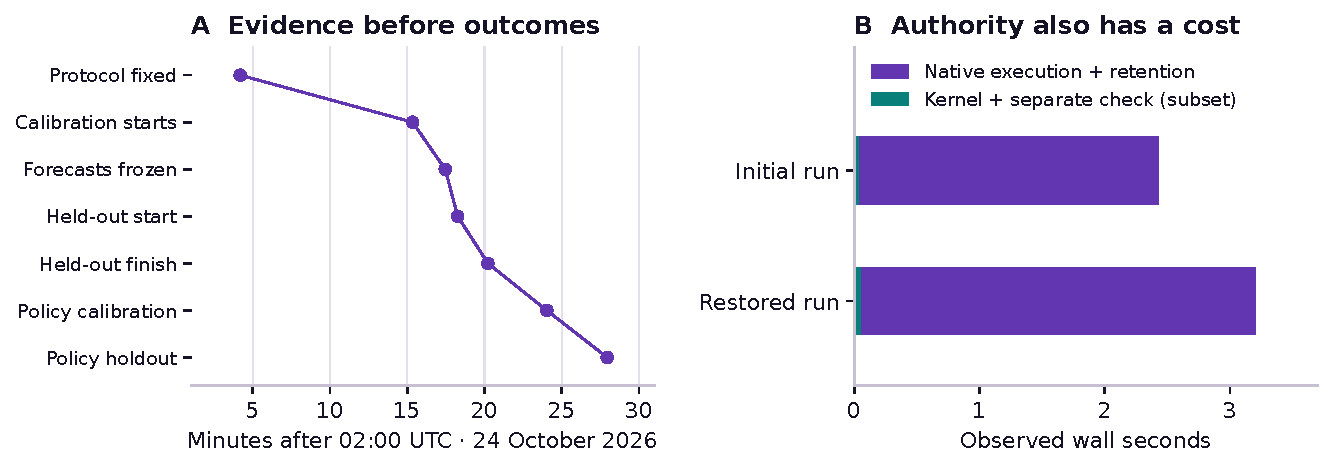
\includegraphics[width=\linewidth]{figures/decision_timeline.pdf}
\caption{\obs{}. (A) Retained protocol, calibration, freeze and confirmation timestamps in UTC document that forecasts preceded execution under the retained hashes. (B) Actual initial and restored native runs; the small colored subsets are numerical handler plus separate checking. The full process also includes startup and bridge work. These are local test-identity executions with no settlement or external authority.}
\label{fig:timeline}\end{figure}

\subsection{The full-cost verdict remains bounded}
The campaign measured 78.516 CPU seconds in numerical calibration and 117.283 in confirmation. The development serialization failure leaves a 9.948-second lower bound for completed batch CPU rather than a complete phase total. Decision calibration and confirmation consume 1.360 and 3.928 child CPU seconds; their policy-model preparation is not a free input to deployed model-using policies. Separate audits and the native process have their own ledger rows. Failure work is retained; validation and late-work subsets are never added twice.

Authoring inference charges, human review, maintenance, external acceptance and opportunity cost are unmetered. These entries are \emph{unknown}, not zero. No live payment, financial transaction, gas use or settled revenue occurred in this study; the hosting/platform charge is not independently known. A firm offer or willingness-to-pay observation is also absent. Consequently, the results establish numerical capability and a bounded model comparison, not positive full-cost commercial Mission Alpha. The detailed ledger retains native time units and makes no token-price or investment-return conversion.
